\documentclass[12pt]{standalone}
\usepackage{tikz}

\begin{document}
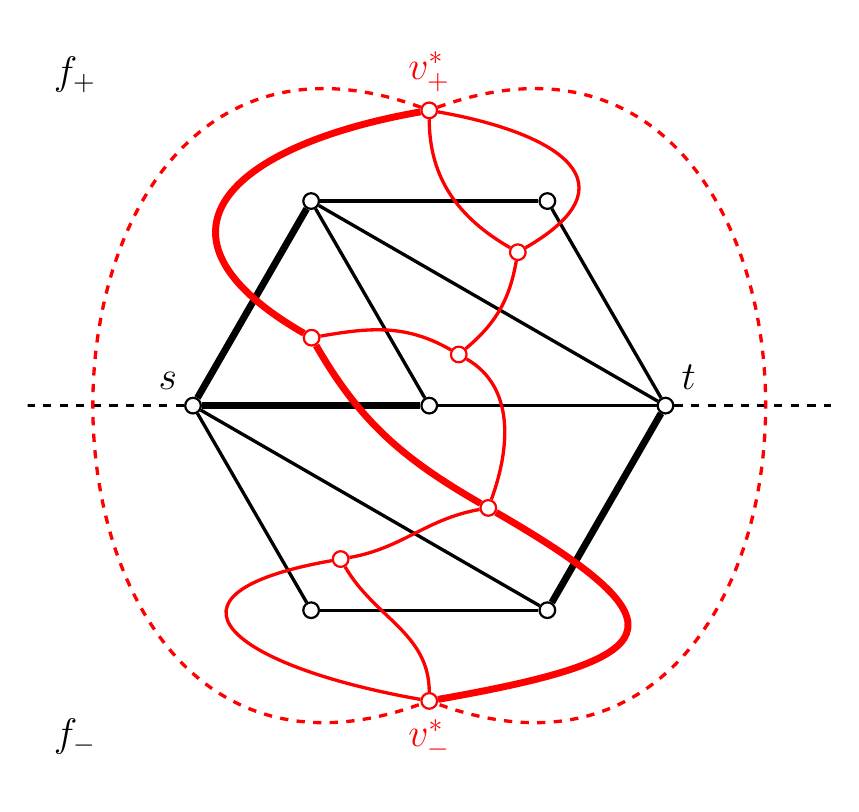
\begin{tikzpicture}[scale=1.5]
    \clip (-3.4,-3.2) rectangle (3.4,3.2);
    \node[circle, thick, draw, inner sep=2pt, label=above right:{\Large $t$}] (a) at (0:2) {};
    \node[circle, thick, draw, inner sep=2pt] (b) at (60:2) {};
    \node[circle, thick, draw, inner sep=2pt] (c) at (120:2) {};
    \node[circle, thick, draw, inner sep=2pt, label=above left:{\Large $s$}] (d) at (180:2) {};
    \node[circle, thick, draw, inner sep=2pt] (e) at (240:2) {};
    \node[circle, thick, draw, inner sep=2pt] (f) at (300:2) {};
    \node[circle, thick, draw, inner sep=2pt] (g) at (0,0) {};
    \draw[very thick, black] (a) -- (b);
    \draw[very thick, black] (a) -- (c);
    \draw[very thick, black] (b) -- (c);
    \draw[line width=2.5pt, black] (c) -- (d);
    \draw[line width=2.5pt, black] (g) -- (d);
    \draw[very thick, black] (a) -- (g);
    \draw[very thick, black] (d) -- (e);
    \draw[very thick, black] (e) -- (f);
    \draw[line width=2.5pt, black] (a) -- (f);
    \draw[very thick, black] (c) -- (g);
    \draw[very thick, black] (d) -- (f);
    \draw[very thick, black, dashed] (a) -- ++(2,0);
    \draw[very thick, black, dashed] (d) -- ++(-2,0);
    \node[circle, thick, draw, inner sep=2pt, red, label={[text=red]above:{\Large $v^*_+$}}] (A) at (0,2.5) {};
    \node[circle, thick, draw, inner sep=2pt, red] (B) at (150:1.15) {};
    \node[circle, thick, draw, inner sep=2pt, red] (C) at (60:0.5) {};
    \node[circle, thick, draw, inner sep=2pt, red] (D) at (60:1.5) {};
    \node[circle, thick, draw, inner sep=2pt, red] (E) at (300:1) {};
    \node[circle, thick, draw, inner sep=2pt, red] (F) at (240:1.5) {};
    \node[circle, thick, draw, inner sep=2pt, red, label={[text=red]below:{\Large $v^*_-$}}] (G) at (0,-2.5) {};
    \draw[line width=2.5pt, red] (A) to[out=190,in=150,looseness=2] (B);
    \draw[very thick, red] (A) to[out=270,in=150,looseness=1] (D);
    \draw[very thick, red] (A) to[out=350,in=30,looseness=2] (D);
    \draw[very thick, red] (B) to[out=10,in=150,looseness=1] (C);
    \draw[very thick, red] (C) to[out=40,in=260,looseness=1] (D);
    \draw[line width=2.5pt, red] (B) to[out=300,in=150,looseness=1] (E);
    \draw[very thick, red] (E) to[out=70,in=330,looseness=1] (C);
    \draw[very thick, red] (E) to[out=190,in=10,looseness=1] (F);
    \draw[very thick, red] (F) to[out=300,in=90,looseness=1] (G);
    \draw[very thick, red] (F) to[out=190,in=170,looseness=3] (G);
    \draw[line width=2.5pt, red] (E) to[out=330,in=10,looseness=3] (G);
    \draw[very thick, red, dashed] (A) to[out=160,in=200,looseness=2] (G);
    \draw[very thick, red, dashed] (A) to[out=20,in=340,looseness=2] (G);
    \node at (-3,2.8) {\Large $f_+$};
    \node at (-3,-2.8) {\Large $f_-$};
\end{tikzpicture}
\end{document}
